\chapter{Amplificadores Operacionais}

Para cada componente podemos trabalhar com vários modelos de diversas complexidades. 
Modelos simples são mais fáceis de trabalhar mas podem esconder diversos fenômenos. 
O ideal será sempre escolher o modelo mais simples mas que ainda sim satisfaça todos os nossos requerimentos.\\
E este é um dos desafios de um engenheiro, dado um problema ponderar qual é 
o modelo mais adequado para se aplicar.

No caso de um Amplificador Operacional (\emph{AmpOp} ou \emph{OpAmp}), um modelo suficientemente
complicado seria o da Figura~\ref{fig:741schematic} que leva em conta a interação de vários transistores.
No entanto, seu equacionamento é complexo, o que nos levaria ao uso de simuladores. Assim, a priori usaremos um 
modelo simplificado para Amplificadores Operacionais.

\begin{figure}[htpb]
  \centering
  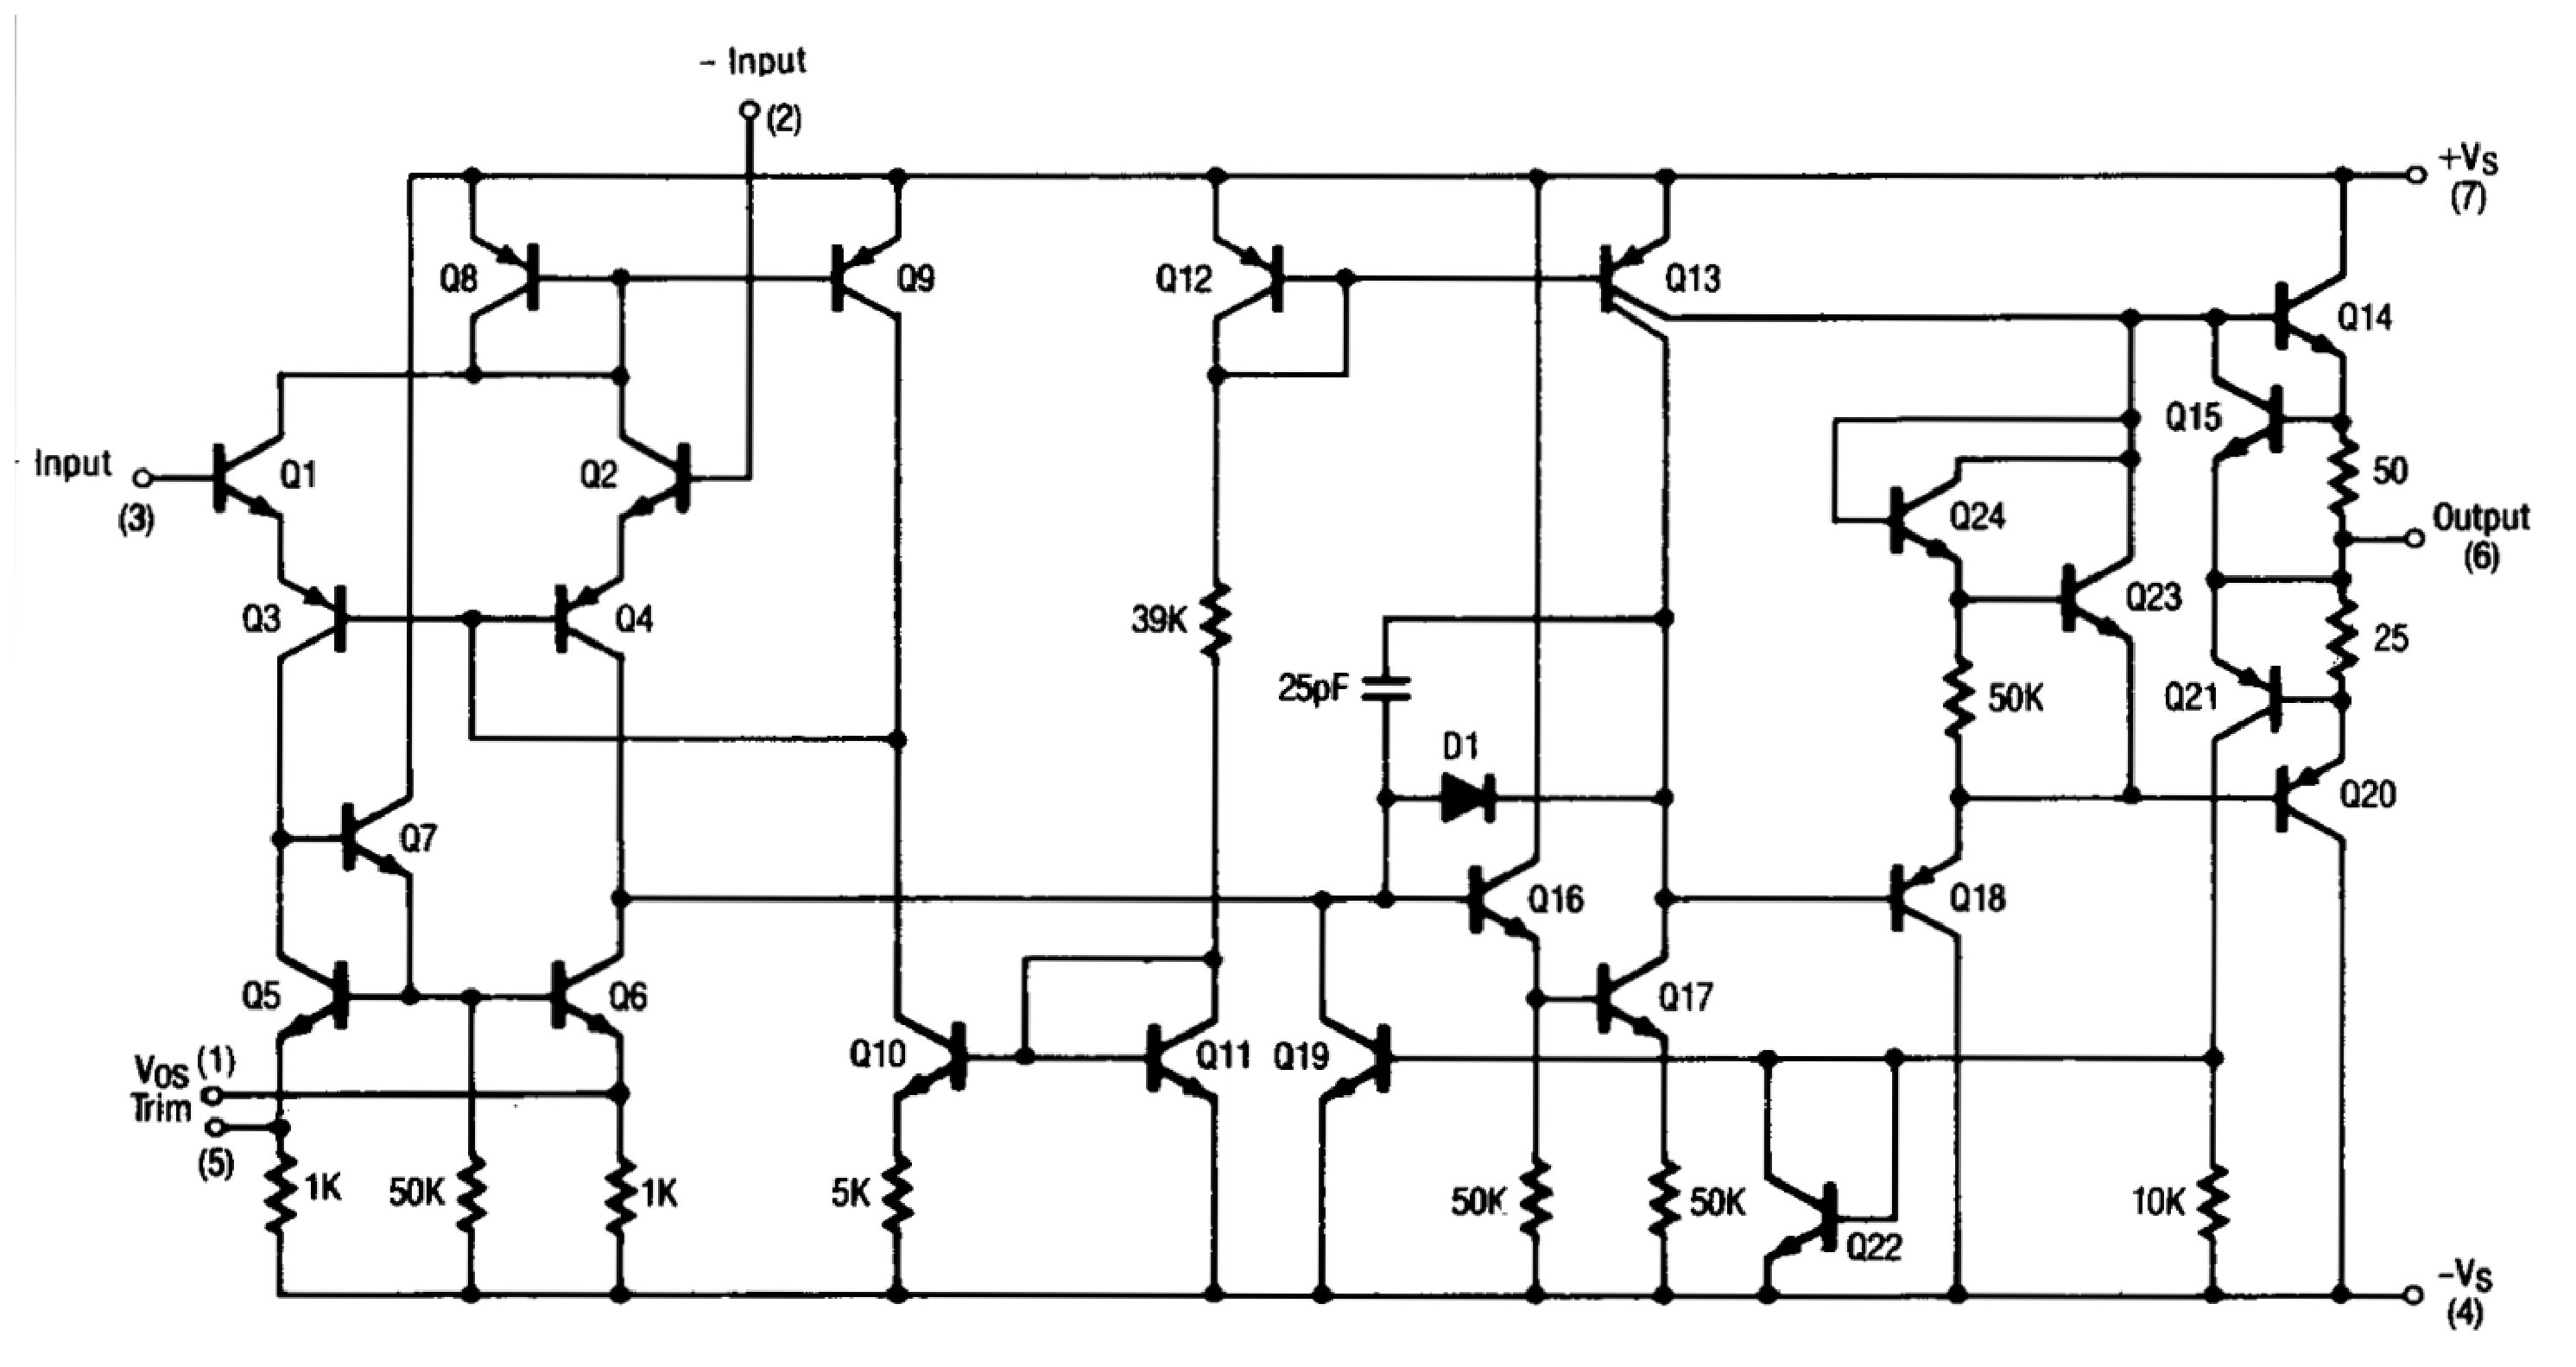
\includegraphics[width=0.8\linewidth]{./Assets/Images/Circuits/AmpOp/741schematic}
  \caption{Esquemático do \emph{AmpOp} 741, retirado do post ``Ubiquituos 741'' do blog ``Ken Shirriff\'s Blog''.}
  \label{fig:741schematic}
\end{figure}

A grosso modo temos dois tipos de transistores bipolar. O transistor PNP e o NPN, conforme mostra a Figura~\ref{placeholder}.


Dado dois sinais de entrada, conforme ilustrado na Figura~\ref{placeholder}, um em cada terminal podemos fazer algumas definições. A tensão de modo comum pode ser definida 
como:

\begin{align}
  V_{CM}  \triangleq \frac{V_{+}+V_{-}}{2} 
\end{align}

E a tensão diferencial como:

\begin{align}
  V_{D} \triangleq V_{+}-V_{-}
\end{align}

Rearranjando as duas equações anteriores, temos:
\begin{align}
  V_{+}  = V_{CM} + V_{D} \\
  V_{-}  = V_{CM} - V_{D}
\end{align}

Representação:
\begin{figure}[htpb]
  \centering
  % \includegraphics[width=0.8\linewidth]{}
  \caption{Onde $G_D$ é o ganho diferencial e $G_{CM}$ é o ganho de modo comum.}
  \label{fig:name}
\end{figure}

Um AmpOp exige que o ganho de modo comum, $G_{CM}$, seja bem inferior ao ganho diferencial, ou seja $G_{D}\gg G_{CM}$,
pois deseja-se amplificar apenas a diferença de seus terminais. Vale lembrar que $G_{D}$ e $G_{CM}$ não são termos 
constantes e variam em função da frequência, o que nos leva a escrever de forma realista:
\begin{align*}
  V_{out}  = G_{D}(f) V_{D} + G_{CM}(f) V_{CM}
\end{align*}
\begin{figure}[htpb]
  \centering
  % \includegraphics[width=0.8\linewidth]{name.ext}
  \caption{Ganho diferencial típico de um AmpOp.}
  \label{fig:name}
\end{figure}
No entanto, quando estivermos trabalhando em \emph{DC}, usaremos $G_{D}$ e $G_{CM}$ 
constantes, pois a frequência é próxima de zero e esta é a modelagem mais simples.
\subsection{Modelo de um AmpOp Ideal}
\begin{figure}[htpb]
  \centering
  % \includegraphics[width=0.8\linewidth]{name.ext}
  \caption{Name}
  \label{fig:name}
\end{figure}

Um AmpOp ideal tem as seguintes propriedades:

